% Provenance (never printed): see sources/outline_sources.md (Year 3:
% ocean dynamics: the Ekman layer derived, the Sverdrup balance, western
% intensification, the abyssal circulation, ocean tides).
% Brief: sources/book5/BRIEFS.md, ch. 21. Curves from
% figdata/bachelor-3/wind_driven_gyre.py and tides.py. Exercise and problem
% values in the Book 5 scratch calculator calc/ch21.py. The basins, winds
% and stations of the exercises and the problem are invented.
\chapter{Ocean Dynamics}\label{ch:b3:ocean-dynamics}

Through the Strait of Florida the Gulf Stream carries about
\qty{32}{\sverdrup} of water northward, and it grows as it follows the coast
north, to about \qty{150}{\sverdrup} near \ang{40} N. On the other side of the same ocean, off Portugal and north
Africa, nothing like it flows south: the water that the Gulf Stream carries
north returns towards the equator as a slow, broad drift across thousands
of kilometres of open sea. Every ocean basin of the Northern Hemisphere has
the same lopsided shape, its fast current on the western side. The
asymmetry follows from the wind, from the friction of the sea, and from one
fact about the Earth: the Coriolis parameter grows towards the pole.
% ledger: rapid:transports (31.7 Sv, rounded), stewart:north-atlantic

\begin{recall}
The tidal force of the Moon and the Sun, spring and neap tides, are in the
physics books. The wind stress, the Ekman layer, the Ekman transport and
the Ekman spiral, upwelling and downwelling, the gyres, the western
boundary currents, the sverdrup ($\qty{1}{\sverdrup} =
\qty{e6}{m^3/s}$), the meridional overturning circulation and the
formation of deep water are in the Year~1 volume, in its chapter on the
ocean circulation; there the wind stress is written $\vec T$, here
$\vec\tau$. The Coriolis parameter, the $\beta$-plane, the Rossby radius
and the geostrophic balance are in Chapter~\ref{ch:b3:gfd-foundations};
vorticity and \omterm{def:b3:atmospheric-dynamics:pv}{potential vorticity} in Chapter~\ref{ch:b3:atmospheric-dynamics}.
\end{recall}

\section{The Ekman layer derived}\label{sec:b3:ocean-dynamics:ekman}

In the Year~1 volume the Ekman transport was found from a balance of forces
on the whole layer, and the spiral of velocities inside it was stated. With
a turbulent friction of constant eddy viscosity $A_z$, the spiral follows
from the equations in a few lines. Write the horizontal velocity as a
complex number, $W = u + \mathrm iv$, and the wind stress as $\tau =
\tau_x + \mathrm i\tau_y$; a multiplication by $-\mathrm i$ turns a vector
by \ang{90} clockwise, to its right seen from above.

\begin{theorem}[Velocity profile of a steady wind-driven surface layer]\label{thm:b3:ocean-dynamics:ekman}
In a steady, horizontally uniform ocean of great depth and constant density
$\rho$, with a constant vertical eddy viscosity $A_z$ and the Coriolis
parameter $f > 0$, the current driven by a wind stress $\tau$ is
\[
W(z) = W_0\,\mathrm e^{(1+\mathrm i)z/\delta},\qquad
W_0 = \frac{\tau}{\rho\sqrt{fA_z}}\,\mathrm e^{-\mathrm i\pi/4},\qquad
\delta = \sqrt{\frac{2A_z}{f}} ,
\]
for $z \le 0$. The surface current is turned \ang{45} to the right of the
stress; with depth it turns further right and decays as $\mathrm
e^{z/\delta}$; the total transport $\int_{-\infty}^0 W\,\mathrm dz =
-\mathrm i\tau/(\rho f)$ is at right angles to the right of the stress.
\end{theorem}

\begin{proof}
Away from coasts there is no horizontal pressure gradient in the layer,
and the Coriolis force balances the friction: $-fv = A_z u''$ and $fu =
A_z v''$, the primes being derivatives in $z$. Multiplying the second by
$\mathrm i$ and adding gives $A_zW'' = \mathrm ifW$. Its solutions are
$\mathrm e^{\pm(1+\mathrm i)z/\delta}$, since $(1+\mathrm i)^2/\delta^2 =
2\mathrm i/\delta^2 = \mathrm if/A_z$; only the plus sign stays bounded as
$z \to -\infty$. At the surface the stress is carried by the friction,
$\rho A_zW'(0) = \tau$, so $W_0 = \tau\delta/(\rho A_z(1+\mathrm i))$.
As $\delta/(\sqrt2 A_z) = 1/\sqrt{fA_z}$ and $1/(1+\mathrm i) = \mathrm
e^{-\mathrm i\pi/4}/\sqrt2$, this is the stated $W_0$. The factor
$\mathrm e^{\mathrm iz/\delta}$ turns clockwise as $z$ decreases. Finally
$\int_{-\infty}^0 W\,\mathrm dz = W_0\delta/(1+\mathrm i) =
\tau\delta^2/(\rho A_z(1+\mathrm i)^2) = \tau\delta^2/(2\mathrm i\rho A_z)
= -\mathrm i\tau/(\rho f)$.
\end{proof}

The theorem recovers both results of the Year~1 volume: Ekman's surface
current at \ang{45} and the transport $\tau/(\rho f)$, at right angles to
the stress and independent of $A_z$, which is never well known. At the
depth $\pi\delta$ the current flows against the surface current, reduced
by $\mathrm e^{-\pi}$, to \qty{4}{\percent}.

\begin{definition}[Ekman depth; Ekman pumping]\label{def:b3:ocean-dynamics:ekman-pumping}
The \emph{Ekman depth}\index{Ekman depth} is $D_E = \pi\delta =
\pi\sqrt{2A_z/f}$, the depth at which the current of the Ekman spiral
flows opposite to the surface current; it measures the thickness of the
Ekman layer. \emph{Ekman pumping}\index{Ekman pumping} is the vertical
velocity $w_E$ at the base of the Ekman layer forced by the convergence or
divergence of the Ekman transport: downward where the transports
converge, upward, sometimes called Ekman suction, where they diverge.
\end{definition}

\begin{proposition}[Ekman pumping]\label{prop:b3:ocean-dynamics:pumping}
With the vertical velocity zero at the sea surface, the \omterm{def:b3:ocean-dynamics:ekman-pumping}{Ekman pumping} is
\[
w_E = \operatorname{curl}_z\frac{\vec\tau}{\rho f}
= \frac{1}{\rho f}\Big(\frac{\partial\tau_y}{\partial x} -
\frac{\partial\tau_x}{\partial y}\Big) + \frac{\beta\tau_x}{\rho f^2} ,
\]
upward positive.
\end{proposition}

\begin{proof}
The volume transport of the layer is $(U_E, V_E) = (\tau_y,
-\tau_x)/(\rho f)$, the theorem written in components. Integrating the
continuity equation $\partial w/\partial z = -(\partial u/\partial x +
\partial v/\partial y)$ through the layer, $w(0) - w_E = -(\partial
U_E/\partial x + \partial V_E/\partial y)$, so $w_E = \partial_x(\tau_y/\rho
f) - \partial_y(\tau_x/\rho f)$. Expanding with $\mathrm df/\mathrm dy =
\beta$ gives the second form.
\end{proof}

A wind that turns cyclonically over the sea, its curl positive, draws
water up from below the layer; an anticyclonic wind pushes it down. Over
the subtropical oceans the trade winds blow from the east on the
equatorward side, the westerlies from the west on the poleward side. Their Ekman
transports, north under the trades and south under the westerlies,
converge between them: the surface water piles up and is pumped down, as
in the figure below. Along a coast where the
wind blows with the coast on its left (in the Northern Hemisphere), the
transport leaves the shore and the coastal upwelling of the Year~1 volume
is Ekman suction concentrated against a wall.

\begin{omfigure}
\centering
\begin{tikzpicture}[>=stealth, font=\small, x=1.1cm, y=1cm]
\fill[omThm!7] (-5,0) rectangle (5,-3.6);
\draw[thick] (-5,0) -- (5,0);
\draw[black!45, densely dashed] (-5,-0.9) -- (5,-0.9);
\node[font=\scriptsize, black!60, anchor=north east, inner sep=1pt] at (4.95,-0.95) {Ekman layer};
% winds: west is out of the page, east into the page
\foreach \x in {-4.2,-3.4,-2.6} {\draw (\x,0.55) circle (0.13); \fill (\x,0.55) circle (0.04);}
\foreach \x in {2.6,3.4,4.2} {\draw (\x,0.55) circle (0.13);
  \draw (\x-0.09,0.46) -- (\x+0.09,0.64); \draw (\x-0.09,0.64) -- (\x+0.09,0.46);}
\node[above] at (-3.4,0.75) {trade winds, from the east};
\node[above] at (3.4,0.75) {westerlies, from the west};
% Ekman transports converge
\draw[->, omDef, very thick] (-4.5,-0.45) -- (-1.2,-0.45);
\draw[->, omDef, very thick] (4.5,-0.45) -- (1.2,-0.45);
\node[omDef, font=\scriptsize, fill=omThm!7, inner sep=1pt] at (-2.85,-0.72) {Ekman transport};
% pumping
\foreach \x in {-0.6,0,0.6} \draw[->, omThm, thick] (\x,-0.55) -- (\x,-1.55);
\node[omThm, font=\scriptsize, anchor=west] at (0.75,-1.25) {$w_E < 0$};
% squashed column and Sverdrup flow
\draw[thick, black!70] (-0.62,-1.75) rectangle (0.62,-3.1);
\node[font=\scriptsize, black!70, align=center] at (0,-2.42) {column\\squashed};
\draw[->, omMeth, very thick] (-0.75,-2.42) -- (-3.2,-2.42);
\node[omMeth, font=\scriptsize, align=center, above] at (-2.6,-2.40) {Sverdrup flow,\\towards the equator};
\draw[black!45, densely dashed] (-5,-3.3) -- (5,-3.3);
\node[font=\scriptsize, black!60, anchor=south east, inner sep=1pt] at (4.95,-3.28) {base of the wind-driven flow};
\node[below, font=\scriptsize] at (-5,-3.6) {south};
\node[below, font=\scriptsize] at (5,-3.6) {north};
\end{tikzpicture}

\par\smallskip{\small A north--south section through a subtropical gyre
of the Northern Hemisphere, east into the page. The Ekman transports under
the trades and the westerlies converge, the water is pumped down, and the
columns beneath, squashed, move towards the equator, where $f$ is smaller,
to keep their \omterm{def:b3:atmospheric-dynamics:pv}{potential vorticity}.}\label{fig:b3:ocean-dynamics:pumping}
\end{omfigure}

\section{The Sverdrup balance}\label{sec:b3:ocean-dynamics:sverdrup}

Below the Ekman layer the ocean is geostrophic. A column of water that is
squashed by \omterm{def:b3:ocean-dynamics:ekman-pumping}{Ekman pumping} must, to keep its \omterm{def:b3:atmospheric-dynamics:pv}{potential vorticity} $f/h$,
move to where $f$ is smaller: towards the equator. In 1947 H.~U.~Sverdrup
made the argument quantitative for the whole depth of the wind-driven flow.
% ledger: stewart:ekman-layer (Sverdrup 1947)

\begin{theorem}[Sverdrup balance]\label{thm:b3:ocean-dynamics:sverdrup}
In a steady ocean in which the non-linear terms and the lateral friction
are negligible, the interior is geostrophic below the Ekman layer, and the
vertical velocity vanishes at some depth $-H$, the total northward volume
transport per unit width of the wind-driven flow obeys the \emph{Sverdrup
balance}\index{Sverdrup balance}
\[
\beta V = \frac{1}{\rho}\operatorname{curl}_z\vec\tau
= \frac{1}{\rho}\Big(\frac{\partial\tau_y}{\partial x} -
\frac{\partial\tau_x}{\partial y}\Big) .
\]
\end{theorem}

\begin{proof}
In the geostrophic interior $fv_g = \rho^{-1}\partial p/\partial x$ and
$fu_g = -\rho^{-1}\partial p/\partial y$. Hence $\partial_x(fu_g) +
\partial_y(fv_g) = 0$, that is $f(\partial_xu_g + \partial_yv_g) + \beta
v_g = 0$, and with continuity, $\beta v_g = f\,\partial w/\partial z$.
Integrating from $-H$, where $w = 0$, to the base of the Ekman layer,
where $w = w_E$, gives $\beta V_g = fw_E$. By
\cref{prop:b3:ocean-dynamics:pumping}, $fw_E = \rho^{-1}\operatorname{curl}_z
\vec\tau + \beta\tau_x/(\rho f)$. Adding the Ekman transport $V_E =
-\tau_x/(\rho f)$, multiplied by $\beta$, cancels the last term:
$\beta(V_g + V_E) = \rho^{-1}\operatorname{curl}_z\vec\tau$.
\end{proof}

The balance is remarkable for what it does not need: neither the depth of
the flow, nor its vertical structure, nor the eddy viscosity, only the
curl of the wind and $\beta$. Sverdrup derived it from the equations of
motion integrated down to a depth of no motion, and tested it against the
hydrographic sections of the research vessels \emph{Carnegie} and
\emph{Bushnell} in the eastern tropical Pacific, between \ang{34} N and
\ang{10} S, with a depth of no motion at \qty{1000}{m}: the transports
computed from the wind matched those computed from the density field, even
where the currents ran against the wind. Later work with better winds
found the best agreement with a depth of no motion near \qty{500}{m}, and
measurements of the mean stress in the equatorial Pacific in 1999 found the
flow there in \omterm{thm:b3:ocean-dynamics:sverdrup}{Sverdrup balance}. Whether the balance holds everywhere is
harder to show than to assume: almost every theory of the ocean
circulation starts from it.
% ledger: stewart:sverdrup

Take the invented basin of this chapter's problem: between \ang{20} and
\ang{50} N, \qty{6000}{km} wide, under a zonal stress $\tau_x =
-\tau_0\cos(\pi(\varphi - \ang{20})/\ang{30})$ with $\tau_0 =
\qty{0.1}{Pa}$, easterly at \ang{20} N, westerly at \ang{50} N, zero at
\ang{35} N. Over almost all the basin the stress curl is negative: the
water is pumped down, by about \qty{35}{m} a year at \ang{35} N, and the
interior flows south, \qty{4.9}{m^2/s} per metre of width at \ang{35} N,
\qty{29.4}{\sverdrup} across the basin. Computed from the observed winds,
the Sverdrup transport of the North Atlantic subtropical gyre reaches about
\qty{30}{\sverdrup} near \ang{28} N.
% ledger: stewart:north-atlantic (computed in figdata/bachelor-3/wind_driven_gyre.py)

\begin{omfigure}
\begin{tikzpicture}
\begin{groupplot}[group style={group size=3 by 1, horizontal sep=0.45cm, yticklabels at=edge left},
  width=0.37\linewidth, height=0.46\linewidth, ymin=20, ymax=50, ytick={20,25,30,35,40,45,50},
  tick label style={font=\scriptsize}, label style={font=\small}, title style={font=\small}]
\nextgroupplot[xlabel={$\tau_x$ (\unit{Pa})}, ylabel={latitude (\unit{\degree} N)},
  xmin=-0.12, xmax=0.12, xtick={-0.1,0,0.1}, title={wind stress},
  scaled x ticks=false, xticklabel style={/pgf/number format/fixed}]
% computed in figdata/bachelor-3/wind_driven_gyre.py
\addplot[black!50, thin] coordinates {(0,20) (0,50)};
\addplot[omThm, thick] table[x=tau, y=lat] {figdata/out/bachelor-3-wind_driven_gyre-merid.dat};
\nextgroupplot[xlabel={$w_E$ (\unit{m/yr})}, xmin=-45, xmax=12, xtick={-40,-20,0},
  title={Ekman pumping}]
\addplot[black!50, thin] coordinates {(0,20) (0,50)};
\addplot[omDef, thick] table[x=wE, y=lat] {figdata/out/bachelor-3-wind_driven_gyre-merid.dat};
\nextgroupplot[xlabel={transport (\unit{\sverdrup})}, xmin=-32, xmax=10, xtick={-30,-20,-10,0,10},
  title={Sverdrup}]
\addplot[black!50, thin] coordinates {(0,20) (0,50)};
\addplot[omMeth, thick] table[x=Vtot, y=lat] {figdata/out/bachelor-3-wind_driven_gyre-merid.dat};
\end{groupplot}
\end{tikzpicture}

\par\smallskip{\small The invented basin of the problem, \ang{20} to
\ang{50} N and \qty{6000}{km} wide. Left, the zonal wind stress, eastward
positive. Centre, the \omterm{def:b3:ocean-dynamics:ekman-pumping}{Ekman pumping}, upward positive: the water is pushed
down south of \ang{47} N, most strongly in the south, where $f$ is small,
and drawn up north of it. Right, the total northward Sverdrup transport across the basin:
the interior goes south, \qty{29.4}{\sverdrup} at \ang{35} N, except in a
thin band at the northern edge, where the stress curl changes sign.}\label{fig:b3:ocean-dynamics:sverdrup}
\end{omfigure}
% ledger: earth:Rmean, geod5:grs80-defining

The Sverdrup transport fixes $V$ at every point, but a streamfunction
needs a boundary condition, and a meridional wall can take only one. If the
interior satisfies no flow through the eastern wall, the southward flow
has nowhere to go at the western wall; the mass is returned by a current
that Sverdrup's equations, without friction, cannot describe.

\section{Western intensification}\label{sec:b3:ocean-dynamics:western}

In 1948 H.~Stommel added the simplest friction to the simplest ocean, and
found the return flow crowded against the western wall, as in the
Year~1 volume's figure of his gyre. He found it only with a Coriolis
parameter that grows northward: with no rotation, or with a uniform one,
his gyre was symmetric.
% ledger: stewart:stommel, stommel:1948

\begin{definition}[Western intensification; Stommel model; Munk boundary layer]\label{def:b3:ocean-dynamics:western-intensification}
\emph{Western intensification}\index{western intensification} is the
crowding of the return flow of a wind-driven gyre into a narrow, fast
current against the western side of the basin. The \emph{Stommel
model}\index{Stommel model} is a homogeneous ocean of constant depth in a
rectangular basin, driven by a zonal wind stress and slowed by a bottom
friction proportional to the depth-integrated velocity, with a rate $r$;
its transport streamfunction $\psi$ ($U = -\partial\psi/\partial y$, $V =
\partial\psi/\partial x$) obeys
\[
r\nabla^2\psi + \beta\frac{\partial\psi}{\partial x} =
\frac{1}{\rho}\operatorname{curl}_z\vec\tau ,\qquad \psi = 0 \text{ on the walls.}
\]
The \emph{Munk boundary layer}\index{Munk boundary layer} is the western
boundary layer of the same gyre when a lateral eddy viscosity $A_H$
replaces the bottom friction; its width scale is $\delta_M =
(A_H/\beta)^{1/3}$.
\end{definition}

The equation is the \omterm{thm:b3:ocean-dynamics:sverdrup}{Sverdrup balance} with the curl of the bottom friction
added: integrated over the depth, $\beta V = \rho^{-1}\operatorname{curl}_z
\vec\tau - r\zeta_T$, where $\zeta_T = \nabla^2\psi$ is the vorticity of
the transport.

\begin{theorem}[Western boundary layer of the Stommel gyre]\label{thm:b3:ocean-dynamics:stommel}
In a basin $0 \le x \le X$, $0 \le y \le L$, with $\tau_x = -\tau_0
\cos(\pi y/L)$ and $\delta_S = r/\beta \ll X$, the Stommel streamfunction
is, to leading order in $\delta_S/X$,
\[
\psi = A\sin\frac{\pi y}{L}\Big[(X - x) - X\mathrm e^{-x/\delta_S}\Big],
\qquad A = \frac{\pi\tau_0}{\rho\beta L} .
\]
The interior carries $AX\sin(\pi y/L)$ south; a boundary layer of width
$\delta_S$ against the western wall returns it north; no boundary layer can
exist against the eastern wall.
\end{theorem}

\begin{proof}
The stress curl is $-\partial\tau_x/\partial y = -(\pi\tau_0/L)\sin(\pi
y/L)$. Over the width of the basin the friction term is smaller than the
$\beta$ term by $\delta_S/X$; dropping it leaves the \omterm{thm:b3:ocean-dynamics:sverdrup}{Sverdrup balance},
$\beta\,\partial\psi/\partial x = -(\pi\tau_0/\rho L)\sin(\pi y/L)$, whose
solution vanishing at $x = X$ is $\psi_I = A\sin(\pi y/L)(X - x)$. It does
not vanish at $x = 0$. Near a wall $\psi$ varies fast in $x$, and the
equation reduces to $r\,\partial^2\psi/\partial x^2 + \beta\,\partial\psi/
\partial x = 0$ for the correction, whose solutions are a constant and
$\mathrm e^{-x/\delta_S}$. This one decays eastward, away from the western
wall: adding $-AX\sin(\pi y/L)\,\mathrm e^{-x/\delta_S}$ makes $\psi = 0$
at $x = 0$ and changes nothing in the interior. At the eastern wall a
correction would have to decay westward, away from $x = X$, and
$\mathrm e^{-x/\delta_S}$ grows westward: there is no such layer, so the
interior must meet the eastern wall by itself, as $\psi_I$ does. The
northward transport between the wall and the point where $V$ changes sign
is $\psi$ there, close to $AX\sin(\pi y/L)$.
\end{proof}

The same answer comes from vorticity. Over the interior the wind gives
each column negative vorticity, and the column pays for it by moving
south, to smaller $f$. On the way back north it gains \omterm{def:b3:atmospheric-dynamics:vorticity-kinds}{planetary vorticity}
and must lose it, which only friction can do. In a northward current
whose speed falls off eastward from near the western wall, $\partial
v/\partial x < 0$ over most of its width: the current's vorticity is negative, and friction, acting against
it, supplies the positive vorticity that the columns need. A northward
current against an eastern wall would have positive vorticity, and
friction would take away the wrong sign.

\begin{omfigure}
\begin{tikzpicture}
\begin{groupplot}[group style={group size=2 by 1, horizontal sep=1.7cm},
  width=0.48\linewidth, height=0.42\linewidth, xmin=0, xmax=400,
  xlabel={distance from the western wall (\unit{km})},
  tick label style={font=\scriptsize}, label style={font=\small},
  legend style={font=\scriptsize, draw=none, fill=none}]
\nextgroupplot[ylabel={$V$ (\unit{m^2/s})}, ymin=-80, ymax=600, legend pos=north east,
  legend cell align=left]
% computed in figdata/bachelor-3/wind_driven_gyre.py
\addplot[omThm, thick] table[x=x, y=vS] {figdata/out/bachelor-3-wind_driven_gyre-bl.dat};
\addlegendentry{Stommel, $\delta_S = \qty{53}{km}$}
\addplot[omDef, thick] table[x=x, y=vM] {figdata/out/bachelor-3-wind_driven_gyre-bl.dat};
\addlegendentry{Munk, $\delta_M = \qty{64}{km}$}
\addplot[black!50, thin, forget plot] coordinates {(0,0) (400,0)};
\nextgroupplot[ylabel={transport from the wall (\unit{\sverdrup})}, ymin=0, ymax=36,
  legend pos=south east, legend cell align=left]
\addplot[omThm, thick] table[x=x, y=cS] {figdata/out/bachelor-3-wind_driven_gyre-bl.dat};
\addlegendentry{Stommel}
\addplot[omDef, thick] table[x=x, y=cM] {figdata/out/bachelor-3-wind_driven_gyre-bl.dat};
\addlegendentry{Munk}
\addplot[black!60, densely dashed] coordinates {(0,29.4) (400,29.4)};
\addlegendentry{interior, \qty{29.4}{\sverdrup}}
\end{groupplot}
\end{tikzpicture}

\par\smallskip{\small The western boundary layer at mid-basin in the
invented basin of the problem (\ang{35} N, \qty{6000}{km} wide). Left, the
northward transport per unit width: Stommel's layer, with a bottom friction
$r = \qty{e-6}{s^{-1}}$, decays exponentially from the wall; Munk's, with
$A_H = \qty{5e3}{m^2/s}$ and no slip at the wall, rises from zero, peaks
about \qty{80}{km} out and is followed by a weak southward countercurrent.
Right, the transport between the wall and each distance, against the
\qty{29.4}{\sverdrup} that the interior carries south: Stommel's layer
gathers \qty{27.9}{\sverdrup} before its flow turns south, Munk's jet
\qty{33.0}{\sverdrup} before its countercurrent.}\label{fig:b3:ocean-dynamics:boundary}
\end{omfigure}
% ledger: stewart:munk

With $r = \qty{e-6}{s^{-1}}$ at \ang{35} N, $\delta_S = \qty{53}{km}$, and
the northward flow occupies the first \qty{250}{km} from the wall. In 1950
W.~H.~Munk replaced the bottom friction by a lateral eddy viscosity $A_H$,
which acts on the shear within the current; the equation gains a term
$A_H\nabla^4\psi$, and near the western wall the correction becomes
$\mathrm e^{-x/2\delta_M}$ times an oscillation, $\cos(\sqrt3x/2\delta_M)$
and $\sin(\sqrt3x/2\delta_M)$. With $A_H = \qty{5e3}{m^2/s}$ the northward
jet is about \qty{225}{km} wide (\qty{233}{km} in the basin of the figure),
with a weak countercurrent beyond it, a shape close to the Gulf Stream and
the Kuroshio. As in Stommel's layer, the transport of the jet does not
depend on the friction but only on the wind-stress curl, the width of the
basin and $\beta$. From the winds of his time Munk computed
\qty{36}{\sverdrup} for the Gulf Stream and \qty{39}{\sverdrup} for the
Kuroshio, about half the transports then measured; with a better drag
coefficient and finer averages of the stress, \qty{32}{\sverdrup} was found
for the Gulf Stream in 1978. Measured mainly with a submarine cable, the
Gulf Stream in the Strait of Florida has carried \qty{31.7}{\sverdrup} on
average since 2004. Downstream it grows to about \qty{150}{\sverdrup} near
\ang{40} N, and offshore of Cape Hatteras a strong recirculation, which the
linear theory does not contain, spoils the agreement.
% ledger: stewart:munk, rapid:transports, stewart:north-atlantic

\section{The abyssal circulation}\label{sec:b3:ocean-dynamics:abyssal}

The deep ocean is filled from a few places. In the Year~1 volume, deep
water forms where surface water is cooled and made dense in the far North
Atlantic and round Antarctica, and spreads through the basins as North
Atlantic Deep Water and Antarctic Bottom Water. Between 1958 and 1960
H.~Stommel, A.~B.~Arons and A.~J.~Faller asked how it spreads, using the
same vorticity argument as Sverdrup.

\begin{definition}[Stommel--Arons model]\label{def:b3:ocean-dynamics:abyssal}
The \emph{Stommel--Arons model}\index{Stommel--Arons model} of the abyssal
circulation supposes that deep water is supplied by convection at a few
high-latitude sources, that it returns to the upper ocean by a slow, uniform
upwelling $W_0$ through the base of the thermocline, balanced by downward
mixing of heat, and that the interior flow is geostrophic and conserves
\omterm{def:b3:atmospheric-dynamics:pv}{potential vorticity}. The circulation is closed by deep western boundary
currents.
\end{definition}

\begin{proposition}[Poleward interior flow of the abyss]\label{prop:b3:ocean-dynamics:abyssal}
In the \omterm{def:b3:ocean-dynamics:abyssal}{Stommel--Arons model}, over a flat bottom, the depth-integrated
northward transport of the abyssal interior is
\[
V = \frac{f}{\beta}W_0 = a\tan\varphi\,W_0 ,
\]
poleward in both hemispheres when $W_0 > 0$.
\end{proposition}

\begin{proof}
In the geostrophic interior $\beta v = f\,\partial w/\partial z$, as in the
proof of the \omterm{thm:b3:ocean-dynamics:sverdrup}{Sverdrup balance}. Integrating from the flat bottom, where
$w = 0$, to the top of the abyssal layer, where $w = W_0$, gives $\beta V =
fW_0$, and $f/\beta = 2\Omega\sin\varphi\,a/(2\Omega\cos\varphi) =
a\tan\varphi$. In the Southern Hemisphere $\tan\varphi < 0$: the flow is
southward, again poleward.
\end{proof}

The result is counter-intuitive: the abyssal interior flows towards the
sources, not away from them. Stommel and Arons built rotating-tank
experiments to convince themselves. The water from the sources travels
along the western walls, in deep western boundary currents that feed the
interior as they go. In a sector of ocean between the equator and the pole
with the whole source $S_0$ near the pole, the western boundary current
carries $2S_0\sin\varphi$ towards the equator, twice the source at the pole
and nothing at the equator: the excess over $S_0$ is water recirculating
from the interior. The model makes the deep circulation driven by mixing,
not by sinking: without the upwelling, convection would only fill the
abyss with a stagnant pool of cold water. Its transit times range from a
few centuries near the sources to nearly a thousand years in the North
Pacific. Over the real ocean floor the ridges divide the basins, mixing is
strong over rough topography, and the deep flow is far more zonal than the
model's. Its lasting prediction is the deep western boundary current: in
the North Atlantic one returns about \qty{14}{\sverdrup} of water at
\qty{2}{\celsius} to the south, while the Gulf Stream carries the warm
water north.
% ledger: stewart:stommel-arons, stewart:deep-circulation, stewart:heat-conveyor

\begin{omfigure}
\centering
\begin{tikzpicture}[>=stealth, font=\small, scale=0.95]
\fill[omThm!7] (0,0) -- (7,0) -- (4.2,5) -- (2.8,5) -- cycle;
\draw[thick] (0,0) -- (2.8,5) -- (4.2,5) -- (7,0);
\draw[black!45, densely dashed] (0,0) -- (7,0);
\node[below, font=\scriptsize] at (3.5,0) {equator};
\node[above, font=\scriptsize] at (3.5,5) {towards the pole};
\fill[omThm] (3.05,4.6) circle (0.17);
\node[font=\scriptsize, anchor=west, inner sep=1pt] at (3.22,4.6) {$S_0$};
% western boundary current
\draw[->, omThm, very thick] (2.75,4.35) -- (0.35,0.25);
\node[omThm, font=\scriptsize, rotate=60.8, inner sep=1pt] at (0.85,2.45) {deep western boundary current};
% interior poleward flow
\foreach \x/\y in {2.6/0.7, 3.8/0.7, 5.0/0.7, 3.1/1.7, 4.3/1.7, 3.6/2.7, 4.6/2.7} {
  \draw[->, omMeth, thick] (\x,\y) -- ++(0.15,0.65);}
% upwelling dots
\foreach \x/\y in {2.2/1.25, 3.4/1.25, 4.6/1.25, 5.6/1.25, 2.7/2.2, 3.9/2.2, 5.0/2.2, 3.3/3.2, 4.3/3.2, 3.8/3.9} {
  \draw[omDef] (\x,\y) circle (0.09); \fill[omDef] (\x,\y) circle (0.03);}
\node[omMeth, font=\scriptsize, align=left, anchor=west] at (6.45,2.6) {poleward\\interior flow};
\node[omDef, font=\scriptsize, align=left, anchor=west] at (6.6,1.5) {upwelling $W_0$};
\end{tikzpicture}

\par\smallskip{\small The Stommel--Arons abyssal circulation in a sector
of the Northern Hemisphere ocean, seen from above. The deep water sinks at
a source $S_0$ near the pole, runs towards the equator in a deep western
boundary current, and leaks into an interior that flows poleward,
everywhere rising slowly through the thermocline (the dots, upwelling
towards the reader).}\label{fig:b3:ocean-dynamics:stommel-arons}
\end{omfigure}

The interior of the model, like Sverdrup's, is geostrophic, and the
geostrophic currents of the deep sea are measured in the way that
Sverdrup measured his: from the density.

\begin{definition}[Dynamic method]\label{def:b3:ocean-dynamics:dynamic-height}
The \emph{dynamic method}\index{dynamic method} computes the geostrophic
current between two hydrographic stations from the density measured at
both, relative to a reference pressure level where the current is taken to
be zero or known. The \omterm{def:b3:gravity-geodesy:geopotential}{geopotential} distance between two pressure surfaces,
$\int\alpha\,\mathrm dp$ with $\alpha = 1/\rho$ the specific volume, is
split into a standard part, the same at both stations, and the
\emph{\omterm{def:b3:gravity-geodesy:geopotential}{geopotential} anomaly} $\Delta\Phi$; the current at the upper surface,
at right angles to the line between stations $A$ and $B$, a distance $L$
apart, is
\[
v = \frac{\Delta\Phi_B - \Delta\Phi_A}{fL} .
\]
\end{definition}

Why not measure the pressure directly, as meteorologists do? A geostrophic
current of \qty{10}{cm/s} at \ang{30} needs a pressure gradient of
\qty{7.5e-3}{Pa/m}, \qty{750}{Pa} across \qty{100}{km}: the weight of
\qty{7.4}{cm} of sea water. No pressure gauge on the sea floor can be
levelled that well. The density, computed to a few parts per million,
gives instead the slope of one pressure surface relative to another. The
lighter, warmer water lies to the right of the current, looking downstream,
in the Northern Hemisphere. Across the Gulf Stream the surfaces of constant
density change depth by more than a kilometre over \qty{100}{km}.
% ledger: stewart:dynamic-method

\begin{method}[Geostrophic current from two stations]\label{met:b3:ocean-dynamics:dynamic}
\begin{enumerate}
\item At each station, compute the specific-volume anomaly $\delta =
  \alpha(S, T, p) - \alpha(35, 0, p)$ from the measured salinity,
  temperature and pressure.
\item Integrate it from the reference pressure up to each pressure $p$:
  $\Delta\Phi(p) = \int_p^{p_{\text{ref}}}\delta\,\mathrm dp$.
\item At each pressure, $v(p) = (\Delta\Phi_B - \Delta\Phi_A)/(fL)$ is
  the current relative to the reference level, positive with station $B$
  on the right.
\item Add the current at the reference level if it is known, from a float
  drifting there or from the sea-surface slope measured by satellite.
\end{enumerate}
\end{method}

\begin{inthefield}[An array of floats]
\begin{minipage}[t]{0.52\linewidth}\vspace{0pt}
\begin{dated}{2024}
Close to four thousand Argo floats drift through the world ocean. Lowered
over the side of a ship, a float sinks to about \qty{1000}{m} and drifts
there for about nine days; it then sinks to \qty{2000}{m} and rises to
the surface, measuring conductivity, temperature and pressure on the way,
and the cycle starts again about every ten days; Deep Argo floats profile to
\qty{6000}{m}. In July 2024 the array collected its three millionth
profile. From the profiles oceanographers compute the \omterm{def:b3:gravity-geodesy:geopotential}{geopotential}
anomalies of the \omterm{def:b3:ocean-dynamics:dynamic-height}{dynamic method} at every float, and the float's own
displacement between two surfacings gives the mean current at its parking
depth: the reference velocity that Sverdrup had to assume is now measured.
\end{dated}
\end{minipage}\hfill
\begin{minipage}[t]{0.44\linewidth}\vspace{0pt}
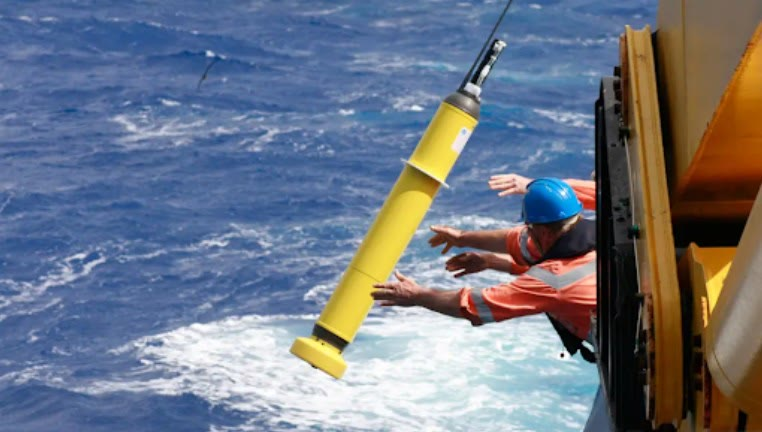
\includegraphics[width=\linewidth]{images/book5/b3-argo-deploy.jpg}

{\scriptsize An Argo float lowered over the side of a research vessel (NOAA
Global Ocean Monitoring and Observing Program, public domain).}
\end{minipage}
\end{inthefield}
% ledger: argo:fleet, noaa:argo-25, photo:b3-argo-deploy

\section{Ocean tides}\label{sec:b3:ocean-dynamics:tides}

Twice a day, a little less than an hour later each day, the sea rises and
falls. The physics books explain the tidal force: the Moon's attraction is
stronger on the near side of the Earth than at its centre, and weaker on the
far side, so that relative to the centre the water is pulled out along the
line to the Moon on both sides.

\begin{definition}[Equilibrium tide; tidal constituent]\label{def:b3:ocean-dynamics:tides}
The \emph{equilibrium tide}\index{equilibrium tide} is the shape that the
surface of an ocean covering the whole Earth would take if it followed the
tide-generating potential instantly, without inertia. A \emph{tidal
constituent}\index{tidal constituent} is one of the harmonic terms, each
with a fixed frequency set by the motions of the Moon and the Sun and an
amplitude and phase found at each place, whose sum makes the tide; they
are named by a letter and the number of cycles per day, such as M$_2$, the
principal lunar semi-diurnal constituent.
\end{definition}

\begin{theorem}[Equilibrium tide of the Moon]\label{thm:b3:ocean-dynamics:equilibrium-tide}
For the Moon, of mass $M$ at distance $d$ from the centre of the Earth, of
mass $M_E$ and radius $a$, the \omterm{def:b3:ocean-dynamics:tides}{equilibrium tide} at an angle $\theta$ from
the point under the Moon is
\[
\eta = K\,\frac{3\cos^2\theta - 1}{2},\qquad
K = \frac{M}{M_E}\Big(\frac{a}{d}\Big)^3 a .
\]
\end{theorem}

\begin{proof}
The potential of the Moon at a point at distance $a$ from the Earth's
centre and angle $\theta$ is $-GM/s$, with $s^2 = d^2 - 2ad\cos\theta +
a^2$. Expanding in $a/d$, $1/s = (1/d)[1 + (a/d)\cos\theta + (a/d)^2
(3\cos^2\theta - 1)/2 + \cdots]$. The first term is a constant; the second
is a uniform field, the one that accelerates the whole Earth in its orbit
round the common centre of mass, and has no effect relative to the Earth.
What is left is the tide-generating potential $\Phi_T = -(GMa^2/d^3)(3
\cos^2\theta - 1)/2$. In equilibrium the sea surface is a surface of
constant total potential, $g\eta + \Phi_T = C$, with $g = GM_E/a^2$, so
$\eta = (M/M_E)(a^4/d^3)(3\cos^2\theta - 1)/2 + C/g$. The mean of
$3\cos^2\theta - 1$ over the sphere is zero; the volume of water being
fixed, $C = 0$.
\end{proof}

With the mass ratio $0.0123$, $d = \qty{384400}{km}$ and $a =
\qty{6371}{km}$, $K = \qty{0.357}{m}$: the sea stands \qty{0.36}{m}
high under the Moon and on the opposite side, and \qty{0.18}{m} low on the
great circle between, a range of \qty{0.54}{m}. At latitude $\varphi$, with
the Moon at declination $\delta$ and at hour angle $H$, $\cos\theta =
\sin\varphi\sin\delta + \cos\varphi\cos\delta\cos H$. As the Earth turns
under the two bulges a place passes through two high waters a lunar day,
\qty{24}{h} \qty{50}{min}: the semi-diurnal tide. When the Moon stands
north or south of the equator the two bulges are tilted, and the two high
waters of a day are unequal, as the figure below shows. The Sun raises a
tide of the same form, \num{0.46} times as large; the two add at new and
full moon, at spring tides, and partly cancel at the quarters.
% ledger: moon5:orbit, earth:Rmean, stewart:tide-equilibrium (computed in figdata/bachelor-3/tides.py)

\begin{omfigure}
\begin{tikzpicture}
\begin{groupplot}[group style={group size=2 by 1, horizontal sep=1.9cm},
  tick label style={font=\scriptsize}, label style={font=\small},
  legend style={font=\scriptsize, draw=none, fill=none}]
\nextgroupplot[width=0.40\linewidth, height=0.40\linewidth, axis equal image, hide axis,
  clip=false, xmin=-1.3, xmax=2.0, ymin=-1.25, ymax=1.25]
% computed in figdata/bachelor-3/tides.py
\addplot[fill=omThm!12, draw=omThm, thick] table[x=x, y=y] {figdata/out/bachelor-3-tides-bulge.dat};
\addplot[black, fill=black!10, domain=0:360, samples=91] ({cos(x)}, {sin(x)});
\draw[->, >=stealth, thick] (axis cs:1.25,0) -- (axis cs:1.95,0);
\node[above, font=\scriptsize, align=center] at (axis cs:1.6,0.08) {to the\\Moon};
\node[font=\scriptsize] at (axis cs:0,0) {Earth};
\nextgroupplot[width=0.54\linewidth, height=0.40\linewidth, xlabel={time (\unit{h})},
  ylabel={$\eta$ (\unit{m})}, xmin=0, xmax=49.6, xtick={0,12,24,36,48}, ymin=-0.2, ymax=0.4,
  legend style={at={(axis cs:12.4,0.39)}, anchor=north}, legend cell align=left, legend columns=2]
\addplot[omDef, thick] table[x=t, y=eta0] {figdata/out/bachelor-3-tides-series.dat};
\addlegendentry{$\delta = 0$}
\addplot[omThm, thick] table[x=t, y=eta20] {figdata/out/bachelor-3-tides-series.dat};
\addlegendentry{$\delta = \ang{20}$}
\addplot[black!50, thin, forget plot] coordinates {(0,0) (49.6,0)};
\end{groupplot}
\end{tikzpicture}

\par\smallskip{\small Left, the \omterm{def:b3:ocean-dynamics:tides}{equilibrium tide} of the Moon, in the plane
that contains the Moon, the bulge exaggerated about two million times.
Right, the \omterm{def:b3:ocean-dynamics:tides}{equilibrium tide} at \ang{45} N over two lunar days, with the
Moon on the equator (blue) and at declination \ang{20} N (red): the second
case has one high water much higher than the other, the diurnal
inequality.}\label{fig:b3:ocean-dynamics:equilibrium-tide}
\end{omfigure}
% ledger: moon5:orbit, stewart:tide-constituents

The harmonic analysis of the \omterm{def:b3:ocean-dynamics:tides}{equilibrium tide} gives its constituents. The
five largest, with their equilibrium amplitudes, are in the table below. At
least 39 constituents are needed to predict a port's tide to a thousandth of
its largest term, and a gauge must run for more than 18.6 years, the period
of the modulation of the lunar tides, to separate them all.

\begin{center}
\small
\begin{tabular}{llrr}
\hline
constituent & origin & period (\unit{h}) & equilibrium amplitude (\unit{m}) \\
\hline
M$_2$ & principal lunar, semi-diurnal & \num{12.4206} & \num{0.2423} \\
S$_2$ & principal solar, semi-diurnal & \num{12.0000} & \num{0.1128} \\
N$_2$ & lunar elliptic, semi-diurnal & \num{12.6584} & \num{0.0464} \\
K$_1$ & luni-solar, diurnal & \num{23.9344} & \num{0.1416} \\
O$_1$ & principal lunar, diurnal & \num{25.8194} & \num{0.1005} \\
\hline
\end{tabular}
\end{center}
% ledger: stewart:tide-constituents, stewart:tide-prediction

The real tide is not the \omterm{def:b3:ocean-dynamics:tides}{equilibrium tide}. To keep a bulge under the Moon
on the equator, the tide would have to travel round the Earth in a lunar
day, at about \qty{460}{m/s}, a speed that a long gravity wave reaches only
in an ocean \qty{22}{km} deep; and the continents stop it. The tide is
instead a forced long wave, sloshing in each basin near resonance, and the
rotation of the Earth makes it turn round the basin.
% ledger: stewart:tide-prediction

\begin{definition}[Kelvin wave]\label{def:b3:ocean-dynamics:kelvin-wave}
An oceanic \emph{Kelvin wave}\index{Kelvin wave} is a long gravity wave
that travels along a coast, or along the equator, with no velocity across
it, its height decreasing exponentially away from the coast over the
Rossby radius. Along a coast it travels with the coast on its right in the
Northern Hemisphere, on its left in the Southern.
\end{definition}

\begin{theorem}[Coastal Kelvin wave]\label{thm:b3:ocean-dynamics:kelvin}
In an ocean of uniform depth $H$ on an $f$-plane, with $f > 0$, bounded by a
straight coast along $y = 0$ and lying in $y > 0$, the linear shallow-water
equations have the solutions with $v = 0$
\[
\eta = \mathrm e^{-y/L_R}F(x - ct),\qquad u = \frac{g}{c}\,\eta,\qquad
c = \sqrt{gH},\quad L_R = \frac{c}{f},
\]
for any profile $F$, and no solution with $v = 0$ travels in the direction
$-x$.
\end{theorem}

\begin{proof}
With $v = 0$ the equations are $\partial u/\partial t = -g\,\partial\eta/
\partial x$, $fu = -g\,\partial\eta/\partial y$ and $\partial\eta/\partial t
+ H\,\partial u/\partial x = 0$. The first and the third give $\partial^2
\eta/\partial t^2 = gH\,\partial^2\eta/\partial x^2$: in $x$ each line
$y = $ const carries waves $F(x \mp ct)$ with $c = \sqrt{gH}$, and then the
first equation gives $u = \pm(g/c)\eta$. The second becomes $\partial\eta/
\partial y = \mp(f/c)\eta$, so $\eta \propto \mathrm e^{\mp y/L_R}$. With
the upper sign the wave decays away from the coast; with the lower one it
would grow without bound into the ocean, which is excluded. The wave goes
towards $+x$ with the ocean on its left, the coast on its right.
\end{proof}

Over the deep ocean, \qty{4000}{m} deep, $c = \qty{198}{m/s}$ and the
Rossby radius is about \qty{2000}{km} at mid-latitudes: the tide sweeps
round a whole basin. Over a shelf sea \qty{50}{m} deep, $c =
\qty{22}{m/s}$, the Rossby radius is under \qty{200}{km}, and an M$_2$
wavelength is about \qty{1000}{km}. In a gulf, the tide entering along one
coast as a \omterm{def:b3:ocean-dynamics:kelvin-wave}{Kelvin wave} returns along the opposite coast, again with the
coast on its right; the two waves cancel at points in between.

\begin{definition}[Amphidromic point; cotidal line; co-range line]\label{def:b3:ocean-dynamics:amphidrome}
An \emph{amphidromic point}\index{amphidromic point} is a point where the
amplitude of a \omterm{def:b3:ocean-dynamics:tides}{tidal constituent} is zero and round which its high water
turns. A \emph{cotidal line}\index{cotidal line} joins the places where a
constituent's high water comes at the same time; a \emph{co-range
line}\index{co-range line} joins the places of equal tidal range. Cotidal
lines radiate from the amphidromic points; co-range lines circle them.
\end{definition}

\begin{omfigure}
\centering
\begin{tikzpicture}
\begin{axis}[width=0.96\linewidth, height=0.35\linewidth, axis equal image,
  xmin=0, xmax=1600, ymin=0, ymax=400, xtick={0,400,800,1200,1600}, ytick={0,200,400},
  xlabel={distance along the channel (\unit{km})}, ylabel={across (\unit{km})},
  tick label style={font=\scriptsize}, label style={font=\small}]
% computed in figdata/bachelor-3/tides.py
\addplot[omDef!70, densely dashed, unbounded coords=jump] table[x=x, y=y] {figdata/out/bachelor-3-tides-cor.dat};
\pgfplotsinvokeforeach{30,60,90,120,150,180,210,240,270,300,330}{
  \addplot[omThm, thin, unbounded coords=jump] table[x=x, y=y] {figdata/out/bachelor-3-tides-cot-#1.dat};
}
\addplot[omThm, very thick, unbounded coords=jump] table[x=x, y=y] {figdata/out/bachelor-3-tides-cot-0.dat};
\addplot[only marks, mark=*, mark size=2pt] table[x=x, y=y] {figdata/out/bachelor-3-tides-amph.dat};
\addplot[->, >=stealth, very thick, domain=20:310, samples=60] ({742.7+70*cos(x)}, {200+70*sin(x)});
\end{axis}
\end{tikzpicture}

\par\smallskip{\small Two \omterm{def:b3:ocean-dynamics:kelvin-wave}{Kelvin waves} of the M$_2$ tide in an invented
channel \qty{400}{km} wide and \qty{50}{m} deep at \ang{55} N, one going
east along the southern coast, the other west along the northern coast.
Red, the \omterm{def:b3:ocean-dynamics:amphidrome}{cotidal lines}, every \ang{30} of phase (about an hour), the
thick one for high water at the time origin; blue dashed, the \omterm{def:b3:ocean-dynamics:amphidrome}{co-range
lines}, every fifth of the amplitude of one wave at its coast. The
\omterm{def:b3:ocean-dynamics:amphidrome}{amphidromic points} (dots) lie on the centre line half a wavelength,
\qty{495}{km}, apart, and the high water turns round them anticlockwise
(arrow).}\label{fig:b3:ocean-dynamics:amphidromes}
\end{omfigure}

The maps of the ocean tide made from satellite altimetry, accurate to about
\qty{2}{cm} in the deep sea, show this structure everywhere: the M$_2$
crest turns anticlockwise round the amphidromes of the Northern Hemisphere
basins and clockwise in the Southern, and the largest ranges are on the
coasts. The tides dissipate \qty{3.75}{TW}, \qty{3.5}{TW} of it in the
ocean, about two thirds of the M$_2$ energy on the shelves and in shallow
seas and one third through internal waves in the deep ocean. That energy
lengthens the day by about \qty{2.07}{ms} a century and pushes the Moon away
by \qty{3.86}{cm} a year; and the part lost in the deep ocean mixes it,
supplying some of the mixing that, in the Stommel--Arons picture, drives
the abyssal circulation.
% ledger: stewart:tide-prediction


\section{Exercises}

\begin{exercise}[$\star$]\label{exo:b3:ocean-dynamics:1}
A westerly wind stress of \qty{0.12}{Pa} blows over the sea at \ang{40} N
($\rho = \qty{1025}{kg/m^3}$, $\Omega = \qty{7.292115e-5}{rad/s}$).
Compute the Ekman volume transport per metre of width and its direction,
and the transport across a section \qty{1000}{km} long, in sverdrups.
\end{exercise}

\begin{exercise}[$\star$]\label{exo:b3:ocean-dynamics:2}
With $A_z = \qty{0.05}{m^2/s}$, compute the \omterm{def:b3:ocean-dynamics:ekman-pumping}{Ekman depth} at \ang{45} N. What
fraction of the surface current remains at that depth?
\end{exercise}

\begin{exercise}[$\star$]\label{exo:b3:ocean-dynamics:3}
At \ang{30} N the curl of the wind stress is \qty{-1e-7}{Pa/m} across a
basin \qty{5000}{km} wide ($a = \qty{6371}{km}$). Compute $\beta$, the
Sverdrup transport per unit width and the total transport, with its
direction.
\end{exercise}

\begin{exercise}[$\star$]\label{exo:b3:ocean-dynamics:4}
From the periods of M$_2$ and S$_2$, compute the period of the cycle of
spring and neap tides, the time between two alignments of the two
constituents.
\end{exercise}

\begin{exercise}[$\star\star$]\label{exo:b3:ocean-dynamics:5}
A westerly stress grows linearly from 0 at \ang{35} N to \qty{0.1}{Pa} at
\ang{45} N, \qty{1110}{km} further north. Compute the \omterm{def:b3:ocean-dynamics:ekman-pumping}{Ekman pumping} at
\ang{40} N, keeping both terms of \cref{prop:b3:ocean-dynamics:pumping}, in
metres per year. Is the water pushed up or down?
\end{exercise}

\begin{exercise}[$\star\star$]\label{exo:b3:ocean-dynamics:6}
In a Stommel gyre with $r = \qty{2e-6}{s^{-1}}$ and $\beta =
\qty{2e-11}{m^{-1}.s^{-1}}$, compute the width $\delta_S$. If the boundary
current carries \qty{30}{\sverdrup} in the upper \qty{800}{m}, within a
width $\delta_S$, what is its mean speed?
\end{exercise}

\begin{exercise}[$\star\star$]\label{exo:b3:ocean-dynamics:7}
Compute the Munk width $\delta_M$ and the width of the northward jet,
$(2\pi/\sqrt3)\,\delta_M$, at \ang{30} N for $A_H = \qty{e4}{m^2/s}$. How
does the width change if $A_H$ is eight times smaller?
\end{exercise}

\begin{exercise}[$\star\star$]\label{exo:b3:ocean-dynamics:8}
Two stations \qty{80}{km} apart lie on a line from west ($A$) to east
($B$) at \ang{36} N. Relative to the \qty{1000}{dbar} surface, the
\omterm{def:b3:gravity-geodesy:geopotential}{geopotential} anomaly of the sea surface is \qty{14.5}{J/kg} at $A$ and
\qty{21.3}{J/kg} at $B$. Compute the surface current relative to
\qty{1000}{dbar} and its direction. Which station has the warmer water
column?
\end{exercise}

\begin{exercise}[$\star\star$]\label{exo:b3:ocean-dynamics:9}
With the \omterm{def:b3:ocean-dynamics:tides}{equilibrium tide} of the Moon, $K = \qty{0.357}{m}$, and the ratio
\num{0.46} of the solar to the lunar tide, compute the equilibrium range
(high water under the bodies minus low water at \ang{90}) at spring and at
neap tides, and their ratio.
\end{exercise}

\begin{exercise}[$\star\star\star$]\label{exo:b3:ocean-dynamics:10}
On the equatorial $\beta$-plane, $f = \beta_0y$ with $\beta_0 =
2\Omega/a$. Show that the \omterm{def:b3:ocean-dynamics:kelvin-wave}{Kelvin wave} $\eta = G(y)F(x - ct)$, $v = 0$,
becomes $G = \exp(-\beta_0y^2/2c)$, trapped on both sides of the equator,
and travels east. Compute its trapping scale $\sqrt{c/\beta_0}$ for a
wave of speed \qty{2.5}{m/s}.
\end{exercise}

\begin{exercise}[$\star\star\star$]\label{exo:b3:ocean-dynamics:11}
(a)~Derive $V = a\tan\varphi\,W_0$ for the abyssal interior from $\beta v =
f\,\partial w/\partial z$. (b)~With $W_0 = \qty{e-7}{m/s}$, compute $V$ at
\ang{30} N and the total poleward transport across a basin
\qty{5000}{km} wide. (c)~Where must the water come from?
\end{exercise}

\begin{exercise}[$\star\star\star$]\label{exo:b3:ocean-dynamics:12}
A geostrophic current $W_g = u_g + \mathrm iv_g$ flows over a flat sea
floor at $z = 0$, with eddy viscosity $A_z$ and no slip at the floor.
(a)~Show that $W = W_g(1 - \mathrm e^{-(1+\mathrm i)z/\delta})$, $\delta =
\sqrt{2A_z/f}$. (b)~Show that the transport defect of this bottom Ekman
layer pumps the vertical velocity $w = \tfrac12\delta\zeta_g$ into the
interior, $\zeta_g$ the vorticity of the geostrophic current. (c)~For
$A_z = \qty{0.01}{m^2/s}$, $f = \qty{e-4}{s^{-1}}$ and an ocean
\qty{4000}{m} deep, compute $\delta$, the spin-down rate $r =
f\delta/2H$, and its inverse in days.
\end{exercise}
% ledger: earth:Rmean, geod5:grs80-defining, stewart:tide-constituents, stewart:tide-equilibrium

\section{Problem: A Gyre in the Sea of Ammar}

\begin{problem}[{Weekend problem --- Ekman pumping, Sverdrup transport,
the western boundary current and the tide of an invented ocean}]
\label{pb:b3:ocean-dynamics:1}
The Sea of Ammar is an invented ocean basin, a rectangle from \ang{20} to
\ang{50} N and \qty{6000}{km} wide, \qty{4000}{m} deep. The wind stress is
zonal, $\tau_x = -\tau_0\cos(\pi(\varphi - \ang{20})/\ang{30})$ with $\tau_0
= \qty{0.1}{Pa}$. Take $\rho = \qty{1025}{kg/m^3}$, $\Omega =
\qty{7.292115e-5}{rad/s}$, $a = \qty{6371}{km}$, $g = \qty{9.81}{m/s^2}$,
and, where a $\beta$-plane is asked for, its value at \ang{35} N.

\medskip\noindent\textbf{Part I --- The Ekman layer.}
\begin{enumerate}
\item Compute the wind stress at \ang{20}, \ang{35} and \ang{50} N.
\item Compute $f$ at the same latitudes.
\item Compute the Ekman volume transport per unit width at \ang{20} and
  \ang{50} N, with its direction. Do the transports converge or diverge in
  the basin?
\item With $A_z = \qty{0.05}{m^2/s}$, compute the \omterm{def:b3:ocean-dynamics:ekman-pumping}{Ekman depth} at \ang{35} N.
\item Compute the \omterm{def:b3:ocean-dynamics:ekman-pumping}{Ekman pumping} at \ang{35} N, in metres per second and per
  year.
\item How many years would it take this pumping to push the surface water
  down \qty{500}{m}?
\end{enumerate}

\medskip\noindent\textbf{Part II --- The Sverdrup interior.}
\begin{enumerate}[resume]
\item Compute the length $L$ of the basin from south to north and $\beta$ at
  \ang{35} N.
\item Compute the curl of the wind stress at \ang{35} N.
\item Compute the Sverdrup transport per unit width at \ang{35} N, with its
  direction.
\item Compute the total interior transport across the basin at \ang{35} N,
  in sverdrups.
\item If this flow is spread through the upper \qty{1000}{m}, what is its
  mean speed, and how many years does a parcel take to move \qty{1000}{km}
  south?
\item Show that $fw_E/\beta$ at \ang{35} N gives the same transport, and
  explain why with the \omterm{def:b3:atmospheric-dynamics:pv}{potential vorticity} of a column.
\end{enumerate}

\medskip\noindent\textbf{Part III --- The western boundary current.}
\begin{enumerate}[resume]
\item Explain why the return flow cannot run along the eastern side of the
  basin.
\item With a bottom friction $r = \qty{e-6}{s^{-1}}$, compute the Stommel
  width $\delta_S$.
\item Compute the northward transport per unit width at the western wall,
  $A(X/\delta_S - 1)$, and the mean speed if it fills the upper
  \qty{1000}{m}.
\item How far from the wall does the northward flow end?
\item Compute the northward transport of the Stommel boundary layer, and
  explain why it falls short of the interior transport by about
  \qty{1.5}{\sverdrup}.
\item With $A_H = \qty{5e3}{m^2/s}$, compute $\delta_M$ and the width of
  Munk's northward jet.
\item Munk's jet carries $1 + \mathrm e^{-\pi/\sqrt3}$ times the interior
  transport. Compute it, and say where the excess goes.
\end{enumerate}

\medskip\noindent\textbf{Part IV --- The tide of the Sea of Ammar.}
\begin{enumerate}[resume]
\item Compute the speed of a \omterm{def:b3:ocean-dynamics:kelvin-wave}{Kelvin wave} in the basin and the Rossby radius
  at \ang{35} N.
\item Compute the wavelength of the M$_2$ \omterm{def:b3:ocean-dynamics:kelvin-wave}{Kelvin wave}.
\item How long does a \omterm{def:b3:ocean-dynamics:kelvin-wave}{Kelvin wave} take to travel once round the coasts of
  the basin, and how many M$_2$ periods is that?
\item At what speed would the \omterm{def:b3:ocean-dynamics:tides}{equilibrium tide} have to travel round the
  \ang{35} N circle to stay under the Moon, and in what depth of ocean
  would a long wave go that fast?
\item Where would you expect the \omterm{def:b3:ocean-dynamics:amphidrome}{amphidromic point} of the basin, and which
  way does high water turn round it?
\item Compute the semi-diurnal equilibrium amplitude at \ang{35} N, $\tfrac34
  K\cos^2\varphi$, with $K = \qty{0.357}{m}$, for the Moon on the equator.
\item Give the transport of the western boundary current that closes the
  gyre of the Sea of Ammar.
\end{enumerate}
\end{problem}
% ledger: earth:Rmean, geod5:grs80-defining, stewart:tide-constituents
